\documentclass[12pt]{jreport}
\usepackage{comment}
\usepackage{./sty/eclepsf}
\usepackage{tascmac}
\usepackage{tabularx}
\usepackage{listliketab}
\usepackage[longnamesfirst]{natbib}
\usepackage[dvipdfmx]{graphics}
\usepackage[dvipdfmx]{graphicx}
\usepackage[dvipdfmx]{color}
\usepackage{subfigure}
\usepackage{alltt}
\usepackage{here}
\usepackage{afterpage}
\usepackage{./sty/ncodeline}
%\usepackage[dvipdfmx, colorlinks, breaklinks,%
\usepackage[dvipdfmx, breaklinks,%
bookmarks=true, bookmarksnumbered=true,%
bookmarkstype=toc, bookmarksopen=true,bookmarksopenlevel=3,%
pdftitle={RG},%
]{hyperref}
\usepackage{bookmark}

\AtBeginDvi{\special{pdf:tounicode EUC-UCS2}}

\usepackage{fancyhdr}

\usepackage{./sty/doxygenorig}

\usepackage{indentfirst}
\usepackage{url}
\usepackage{listings,./sty/jlisting}

\def\lstlistingname{プログラム}

\lstset{%
 language={C++},
 %backgroundcolor={\color[gray]{.85}},%
 basicstyle={\small\ttfamily},%
 identifierstyle={\small},%
 commentstyle={\small\itshape},%
 keywordstyle={\small\bfseries},%
 ndkeywordstyle={\small\ttfamily},%
 stringstyle={\small\ttfamily},
 frame={tb},
 framesep=1zw,
 breaklines=true,
 numbers=left,%
 xrightmargin=0zw,%
 xleftmargin=1.5zw,%
 numberstyle={\scriptsize},%
 stepnumber=1,
 numbersep=1zw,%
 lineskip=-0.5ex%
}

\usepackage{amssymb}
%\usepackage{supertabular,multirow}

\usepackage{array}
\newcolumntype{M}[1]{>{\centering\arraybackslash}m{#1}}

% A4  size: 297mm*210mm %1pt = 0.35mm
\setlength{\topmargin}{-3.4mm} % 10pt 25.4mm - 3.4mm = 22mm
\setlength{\oddsidemargin}{-0.4mm} % 25.4mm - 0.4mm = 25mm
\setlength{\evensidemargin}{-0.4mm} % 25.4mm - 0.4mm = 25mm
\setlength{\textheight}{231mm} % 660pt % original is 225.75mm 645pt
\setlength{\textwidth}{160mm} % 457pt

\renewcommand{\topfraction}{.99}
\renewcommand{\textfraction}{.0}
\renewcommand{\floatpagefraction}{.99}
\renewcommand{\bibname}{参考文献}


\pagestyle{fancy}
\lhead[]{}

\makeatletter
\def\chaptermark#1{\markboth {\ifnum \c@secnumdepth>\m@ne
\@chapapp\ \thechapter \@chappos\ \fi #1}{}}
\makeatother

% タイトル
\def\title{業務用オーディオシステムにおける\\AES67アプリケーションの実装と検証}
% 英語タイトル
\def\etitle{Implementation and Evaluation of AES67 sender and receiver}
% 著者(日本語)
\def\author{城 一統}
% 著者(英語)
\def\eauthor{Kazunori Jo}
% 学部・研究科
\def\dept{慶應義塾大学 環境情報学部}
% 学部・研究科(英語)
\def\edept{Keio University Bachelor of Arts in Environment and Information Studies}

\begin{document}

\pagenumbering{roman}
\begin{titlepage}
  \begin{center}
    \begin{large}
      卒業論文   2019年度(令和元年度)\\
      \vspace{24pt}
      \title
      \end{large}
  \end{center}
  \vspace{40em}
  \begin{flushright}
    \large \dept\\
    \author
  \end{flushright}
\end{titlepage}

\thispagestyle{empty}


卒業論文要旨 - 2019年度 (令和元年度)
\begin{center}
\begin{large}
\begin{tabular}{|M{0.97\linewidth}|}
    \hline
      \title \\
    \hline
\end{tabular}
\end{large}
\end{center}

~ \\

従来のオーディオ伝送の諸問題を解決するために、IPオーディオ伝送が登場した。のちに乱立するさまざまなIPオーディオ伝送規格を標準化するAES67規格が策定された。ブラックボックスとなっている商用規格を使わずとも、自由に機器やアプリケーションを開発することができるようになった。

業務用オーディオシステムに必要な要件は、遅延の少なさ、高音質、伝送の安定性が挙げられる。

遅延を感じ、バイオリンの演奏に支障を与える程度を計測する実験で、10ミリ秒であればほとんどの被験者が遅延を感じないという研究がある。音が入力されてからスピーカーで出力されるまでの遅延時間には、伝送経路以外の時間も含まれる。例えば、ワイヤレスマイクを使用した場合や、エフェクタ等の信号処理で遅延が発生する。よって、オーディオ伝送において遅延を少なくすることが重要だ。DanteとよばれるIPオーディオ伝送規格では、デフォルトで1ミリ秒の遅延を許容する設定になっている。

デジタルオーディオ伝送は、伝送経路において信号の劣化しないため業務用途で頻繁に使われているが、それらは非圧縮で伝送されている。不可逆圧縮する場合、圧縮と展開を繰り返すたびに、劣化してしまう。よって、複雑な信号処理が行われることもある業務用オーディオでは非圧縮伝送は必須条件だ。PCM 48kHz/24bit程度であれば望ましい。

伝送経路の安定性も業務用途によって欠かせない要素である。プロのアーティストによるライブやコンサートでは、一瞬たりとも音が途切れることは許されない。機材トラブルやケーブルの断線が起きれば、オーディオ伝送は行われなくなる。デジタルオーディオ伝送規格では、伝送経路の冗長化をサポートしているものがある。

これらの業務用オーディオシステムに必要な要件を踏まえ、AES67によるソフトウェア実装の実際の業務用オーディオ現場における利用可能性を検証することにした。実装においてGo言語を採用した。移植性の高さと高速に動作するためである。

その結果、遅延量は想定する1ミリ秒を下回り、AES67のソフトウェアオーディオ伝送は、業務用オーディオにおける要件を満たすと考えられる。

~ \\
キーワード:\\
\underline{1. AES67},
\underline{2. Audio over IP}
\begin{flushright}
\dept \\
\author
\end{flushright}

\thispagestyle{plain}
\clearpage

Abstract of Bachelor's Thesis - Academic Year 2019
\begin{center}
\begin{large}
\begin{tabular}{|p{0.97\linewidth}|}
    \hline
      \etitle \\
    \hline
\end{tabular}
\end{large}
\end{center}

~ \\
IP audio transmission has emerged to solve the problems of conventional audio transmission. The AES 67 standard was established to standardize the various IP audio transmission standards that were established later. It is now possible to freely develop devices and applications without using the commercial standard which is a black box.

Requirements for professional audio systems include low latency, high sound quality, and transmission stability.

One study found that most subjects felt no delay at 10 milliseconds when measuring how slow they felt and how difficult it was to play the violin. The delay time from the input of the sound to the output of the speaker includes a time other than the transmission path. For example, when a wireless microphone is used, a delay occurs in signal processing of an effector or the like. Therefore, it is important to reduce the delay in audio transmission. The IP audio transmission standard called Dante allows a delay of 1 millisecond by default.

Digital audio transmissions are frequently used in commercial applications because they do not degrade the signal in the transmission path, but they are transmitted uncompressed. In the case of lossy compression, it deteriorates every time compression and expansion are repeated. Therefore, uncompressed transmission is an essential condition for professional audio, which can perform complex signal processing. It is desirable if the frequency is about 48 kHz/24 bit PCM.

The stability of the transmission path is also an essential element depending on the application. At concerts and concerts by professional artists, the sound cannot be cut off for a moment. If equipment trouble or a cable break occurs, audio transmission is stopped. Some digital audio transmission standards support redundant transmission paths.

Based on the requirements for these professional audio systems, we decided to verify the applicability of AES 67 software implementation in the actual professional audio field. Go language was adopted in the implementation. This is because of its high portability and high speed operation.

As a result, the amount of delay is less than the expected 1 millisecond, and AES 67 software audio transmission is considered to meet the requirements for professional audio.
~ \\
Keywords : \\
\underline{1. AES67},
\underline{2. Audio over IP}
\begin{flushright}
\edept \\
\eauthor
\end{flushright}

\thispagestyle{plain}
\clearpage

\tableofcontents\thispagestyle{plain} %目次
\clearpage
\listoffigures\thispagestyle{plain} %図目次
\clearpage
\listoftables\thispagestyle{plain} %表目次
\clearpage

\pagenumbering{arabic}
\chapter{序論}
\label{chap:introduction}

\section{背景}
\label{section:background}

本論文の読者は、オーディオの伝送と聞いて何を思い浮かべるだろうか。音楽をイヤホンやヘッドホンで聴くこと読者も多いだろう。スマートフォンやコンピュータといった再生機器に、3.5mmステレオミニプラグ(いわゆるイヤホンジャック)を接続するか、あるいはBluetoothといった無線伝送によってオーディオは伝送されている。

一般的な民生用オーディオ伝送では、インターフェイスや接続が手軽な利便性をとり、ある程度の音質劣化や遅延は許容されている。一方で、業務用オーディオの世界では妥協のない高音質の追求や、絶対に伝送される安定性が優先される。

プロのアーティストによるライブ、テレビ局やインターネットの動画配信などで用いられる業務用オーディオでは、民生向けで使われるオーディオ伝送に比べ、次にあげるような条件が要求される。

\begin{itemize}
  \item 高音質
  \item 低遅延
  \item 伝送の安定性
\end{itemize}

デジタル伝送技術は、アナログ伝送に比べ伝送経路による劣化が起こりにくくなっている。ただし、オーディオ入力と出力の最初と最後は図\ref{fig:first_and_last_need_ad_da}のように、必ずアナログとデジタルの変換(以下、A/D変換、D/A変換)が必要となる。そのため、すべての伝送経路をアナログで伝送するのに比べ、少なからず伝送するにあたりA/D変換とD/A変換にともなう遅延が発生する。しかしながら、技術の向上によって遅延量は少なくなっている。たとえば、XXXでA/D、D/A変換に要する時間はX.Xms以内である。

\begin{figure}[htbp]
  \centering
  \label{fig:first_and_last_need_ad_da}
  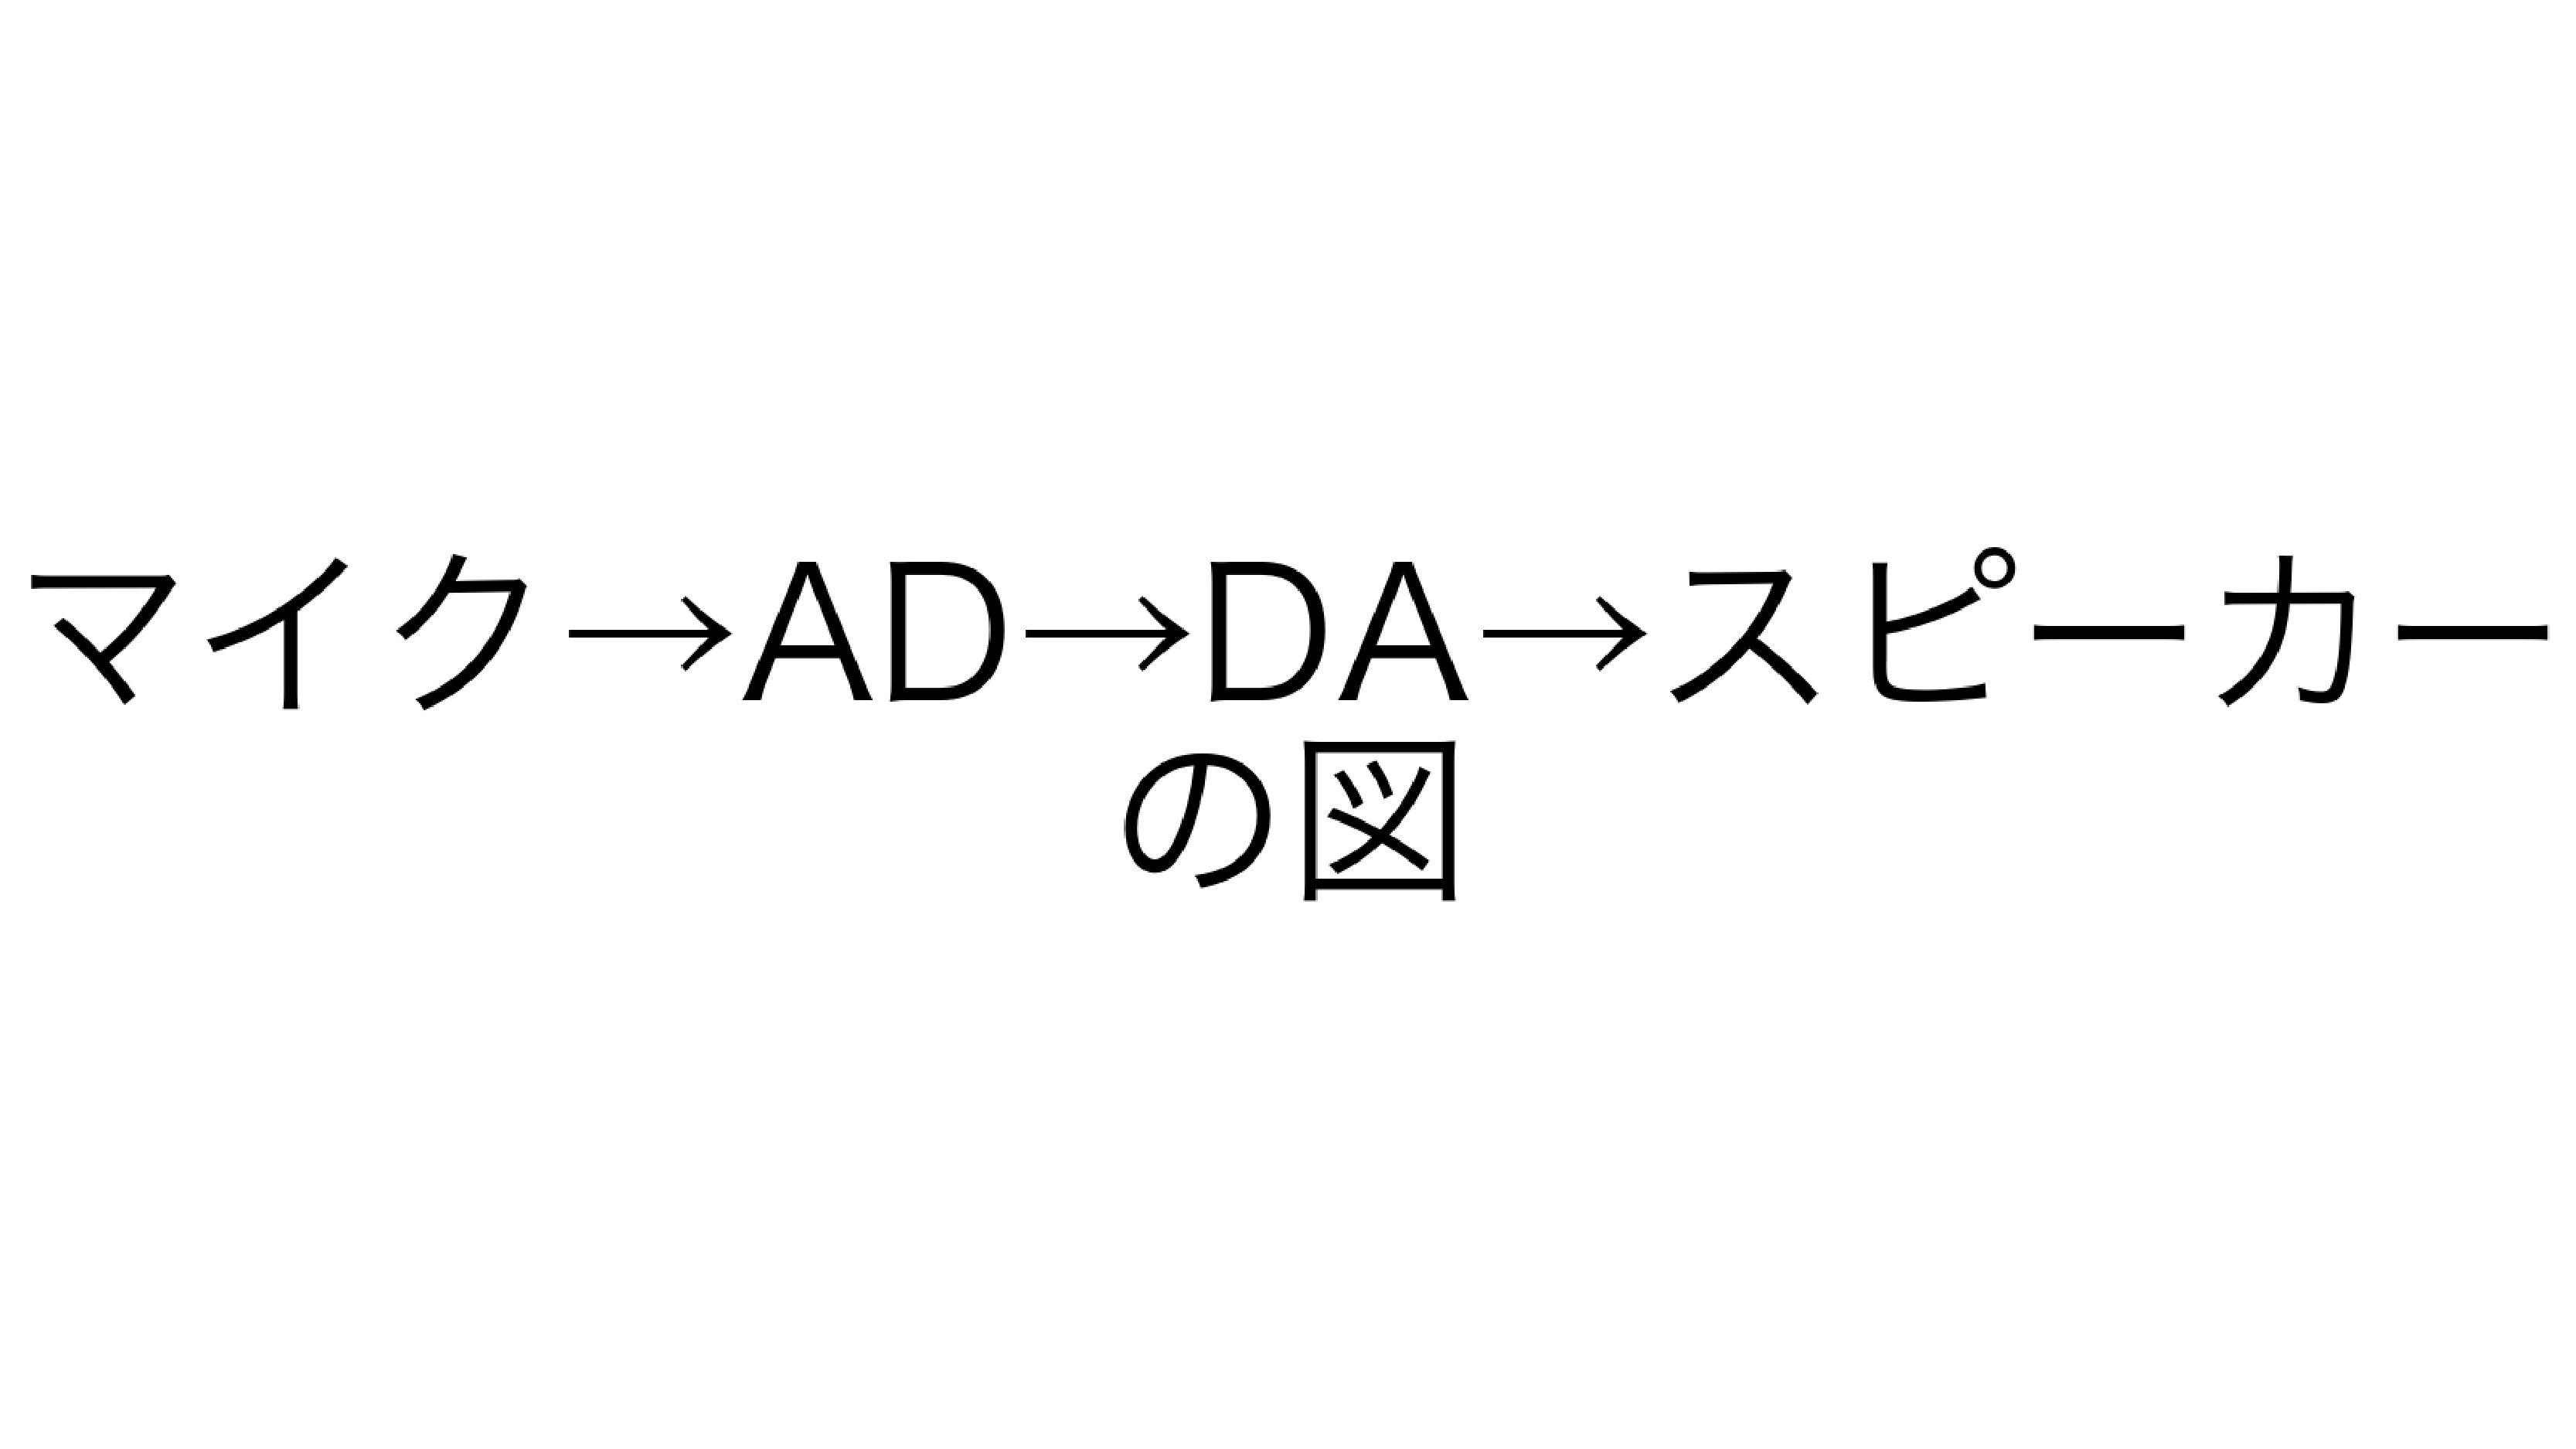
\includegraphics[width=0.8\linewidth]{img/first_and_last_need_ad_da.pdf}
  \caption{マイク→AD→DA→スピーカーの図}
\end{figure}

もう一つ、デジタル伝送を行うことによる恩恵は高音質のまま伝送できることである。アナログ伝送のまま伝送を行えば、理論的にはA/D、D/A変換を挟まないため、劣化しないはずである。しかしながら、アナログ伝送は外部からのノイズに弱く、伝送経路中で劣化する可能性が否定できない。

そこで、デジタル伝送ではアナログ信号を0と1の信号にする。アナログ信号は、連続したデータ表現のため、デジタル信号にそのまま表現すると無限となってしまう。それでは現実的でないためデジタル信号では、量子化によってデータ量を減らすことができる\cite{analog-io}。したがって、従来アナログ伝送においてケーブル1本で1チャンネル伝送していたところをデジタル伝送により2チャンネル以上の多チャンネル伝送ができるようになる。AES/EBUというデジタル伝送規格では、接続に用いるケーブルにもよるが2〜16チャンネル程度(要出典)の伝送が行える。

インターネット、ネットワークの接続に利用するEthernet(イーサネット)は、インターネットの高速化やコンピュータで扱うコンテンツのリッチ化にともない、通信速度の高速化が進んでいる。2019年現在、市販のEthernetケーブル(図\ref{fig:ethernet_cable})を用いた接続では、最大10Gbps\footnote{Gbps: Gigabit per second、ギガビット毎秒}の通信速度で転送することができる。

(余裕があればAES/EBUの転送速度と比較する)

\begin{figure}[htbp]
  \centering
  \label{fig:ethernet_cable}
  
\includegraphics[width=0.4\linewidth]{img/ethernet_cable.pdf}
  \caption{Ethernetケーブル}
\end{figure}

Ethernetを用いたデジタルオーディオ伝送では、高速なEthernetの帯域を用いて従来のデジタルオーディオ伝送に比べ、より多くのチャンネルを伝送することができる。主に、XXXやXXXといった規格がある。多チャンネル化が実現できるのみならず、エラー訂正が可能となる(要出典)。

大規模な業務用オーディオ環境では、広帯域なEthernetを用いたIPベースの伝送への移行が進んでいる。主流となっているのは、Audinate社が開発したDanteという規格だ。Audinate社はDante機能のチップをオーディオ機器メーカーに卸す手法をとっている。オーディオ機器メーカーに対してDanteに関する詳細な仕様(なんの?)は公開されておらず、ブラックボックスとなっている現状がある。したがって、オープンなIPベースのデジタルオーディオ伝送が必要である。

そこで、登場したのがAES67だ。AES67は、乱立する既存のIPベースのデジタルオーディオ伝送技術を共通化し、相互運用性を高めるための規格である。今後、オーディオのIP伝送が主流となっていくなかで、オープンな標準化技術によってさまざまなオーディオ機器を接続できることは重要である。

\section{本論文の目的}

本論文では、オーディオ機器の最初と最後のA/D、D/A変換を行う前のアナログ伝送を除くすべての伝送経路をAES67によって実現できるかの可能性を追求する。必要となる、AES67オーディオストリームを送受信するアプリケーションを実装する。その上で、既存の商用規格から置き換えが可能なのか、業務用途で要求される厳しい条件に耐えられるかを検証する。

\section{本論文の構成}

本論文における以降の構成は次の通りである。

\ref{chap:related_works}章では、本論文で扱うIPベースのオーディオ伝送について理解ための前提技術について、解説する。業務用オーディオが使われている現場の構成、さらにはオーディオのデジタル伝送技術について触れる。

\ref{chap:design}章では、AES67を用いたIPベースのオーディオ伝送の送受信を行うアプリケーションの設計を行い、その内容について述べる。

\ref{chap:implementation}章では、\ref{chap:design}章で設計したアプリケーションを実装し、その内容について述べる。

\ref{chap:evaluation}章では、\ref{chap:implementation}章で実装したアプリケーションをもとに、実際の業務用オーディオ環境を模した実験を行い、評価した結果について述べる。

\ref{chap:conclusion}章では、本研究における結論と今後の展望、業務用オーディオの伝送技術の未来について述べる。

\chapter{関連技術}
\label{chap:related_works}

本章では、本研究と関連するオーディオのデジタル伝送を行う関連技術について、IPベースの伝送とIPベースでない伝送について示す。

\section*{非IPベースのデジタル伝送}

\section{AES/EBU}
\label{sec:aes/ebu}

AES/EBUは、オーディオ専門家の国際組織である米国オーディオ技術者協会(AES)\footnote{Audio Engineering Society, Inc. \url{http://www.aes.org/}}と、欧州放送連合(EBU)\footnote{European Broadcasting Union \url{https://www.ebu.ch/home}}の両者によって策定されたデジタルオーディオ伝送規格である。それぞれAES3-1985\cite{aes3-1985}とEBU Tech.3250-E\cite{ebutech-3250-e}という名称で、1985年に策定された。なお、両者の名前をとって一般的にAES/EBUの名称で呼ばれている。

\subsection{IECによる標準化}

また、AES3は国際電気標準会議(IEC\footnote{International Electrotechnical Commission})によって標準化もされている。IECによる標準化では4つのパートで構成されており、IEC 60958-3ではAES3から派生した民生用途向け(いわゆるS/PDIF)と、IEC 60958-4ではAES3に基づいた業務用途向けのものが定められている。

接続するインターフェイスはIEC規格によって策定されている。アナログオーディオ伝送にも用いられるXLRコネクタによるバランス(平衡)接続や、BNCコネクタを用いた同軸ケーブルによるアンバランス(不平衡)接続、さらにはD-subコネクタを用いたオーディオ機器メーカーによる独自規格が存在する。本稿執筆時点で最新のAES3規格では、光ファイバーによる伝送も検討されている\footnote{AES3-2009 (r2019): AES standard for digital audio engineering - Serial transmission format for two-channel linearly represented digital audio data \url{http://www.aes.org/publications/standards/search.cfm?docID=13}}。

\subsection{AES-3id-1995}

BNCコネクタを用いたアンバランス接続は、AES3-id-1995という名称で策定されている。AES/EBUでは、インピーダンスが110Ωのケーブルを用いる。バランス接続は、ノイズの影響を受けにくく安定した伝送が期待できるものの、アンバランス接続の同軸ケーブルに比べ高価である。BNCコネクタが付いたインピーダンスが75Ωの同軸ケーブルは、業務用ビデオ伝送の分野で主流だ。

大規模なホールのような会場では予めさまざまな場所に配線しておき、パッチ盤で接続するという手法がある。パッチ盤のコネクタがBNCであれば何を伝送してもよいため、ビデオ伝送用に配線されている既存の同軸ケーブルを利用できる。AES/EBUで同軸ケーブルを用いて伝送するというアイデアは、ビデオ技術の団体米国映画テレビ技術者協会(SMPTE)\footnote{Society of Motion Picture and Television Engineers \url{https://www.smpte.org/}}からAESに対して要望が出ていたという経緯がある\cite{aes3id-1995-column}。同軸ケーブルを用いた伝送は、信号を補償(ブースト)することで長距離伝送が可能となる。同規格は、SMPTEからSMPTE 276M-1995という規格にもなっている。

\section{S/PDIF}

前述したとおり、業務用のAES/EBUから派生した民生用向けの規格は、IEC 60958-3によって標準化されている。この規格は、一般的にS/PDIF(Sony/Philips Digital Interface)と呼ばれる。日本のソニーとオランダのフィリップスが開発したためそのように呼ばれている。

AES/EBUでは、民生用では馴染みの薄いXLRコネクタやBNCコネクタが用いられてきたが、S/PDIFでは光デジタル音声端子(Optical)と同軸デジタル音声端子(Coaxial)の2種類が存在する。光デジタル端子は、東芝が提唱したTOSLINKと呼ばれる角型コネクタ、Mini-TOSLINKと呼ばれる3.5mmステレオミニプラグの形状をしたコネクタがある。同軸端子は、RCAコネクタが使われている。

Mini-TOSLINKは、以前AppleのパソコンであるiMacやMac mini、MacBook Proにも搭載されていた\footnote{MacBook Proは2015年発売の機種まで、3.5mmステレオミニジャックにアナログ入力とコンボジャックで搭載していた。 \url{https://support.apple.com/kb/SP719?locale=ja_JP&viewlocale=ja_JP}}。

\subsection{AES/EBUとS/PDIFの違い}

AES/EBUは業務用でS/PDIFは民生用だが、それぞれの違いを表\ref{tab:compare}に記す。業務用オーディオは、可能な限り伝送距離を長くし、XLRコネクタで接続した場合バランス接続による安定性をとっている。一方、民生用オーディオは出力レベルを低くし、伝送距離も10m程度である。ただし、著作権保護信号を伝送することができ、受信機が信号を認識するとその機器で録音ができなくなるようだ。

\begin{table}[htb]
  \begin{minipage}{\textwidth}
    \label{tab:compare}
    \caption{AES/EBUとS/PDIFの比較\cite{aesebuandspdif}}
    \begin{tabular}{c|ccc} \hline
      & AES3-1992 (r1997) & AES-3id-1995\footnote{SMPTE 276M-1995} & S/PDIF\footnote{IEC 60958-3} \\ \hline
      ケーブル & 110Ω STP & 75Ω 同軸 & 75Ω 同軸/光ファイバー \\
      インターフェイス & バランス & アンバランス & アンバランス \\
      コネクタ & 3ピンXLR & BNC & RCA / TOSLINK \\
      信号レベル & 2--7V peak to peak & 1.0--1.2V peak to peak & 0.5--0.6V peak to peak \\
      最小信号レベル & 0.2V & 0.32V & 0.2V \\
      最大伝送距離 & 100m & 1000m & 10m \\
      コピー制御 & 不可 & 不可 & 可能 \\
      ビット深度 & 24bit & 24bit & 20bit(24bitに拡張可能)\footnote{4bit分予備領域として確保されており、20+4bitを合わせて送信できる。} \\
    \end{tabular}
  \end{minipage}
\end{table}

\section{SDI}

SDI\footnote{Serial Digital Interface}は、ビデオ信号を伝送する規格である。非圧縮のビデオとオーディオを伝送することが可能だ。

本来はビデオ伝送用の規格だが、AES3に準拠した48kHz/24bitのオーディオを16チャンネル伝送できる。

\section{CobraNet}

CobraNetは、1996年に米Peak Audioが開発したEthernetを用いたオーディオ伝送規格である。Ethernetを使うが、IPベースでないのが特徴的だ\cite{best-practices-in-network-audio}。

\section*{IPベースのデジタル伝送}

\section{Ethernet AVB}

Ethernet AVBは、IEEE\footnote{Institute of Electrical and Electronics Engineers}により策定されたEthernetでオーディオとビデオを伝送する規格である。正式にはIEEE 802.1 Audio/Video Bridgingという。

\section{Dante}

Danteは、米Audinate\footnote{\url{https://www.audinate.com/?lang=ja}}が開発したIPベースのオーディオ伝送規格である。最大ビット深度は32bit、最大サンプリング周波数は192kHzで伝送できる\cite{best-practices-in-network-audio}。

2019年現在、ミキサーやパワーアンプなど、総合音響機器メーカーのヤマハや\footnote{\url{https://jp.yamaha.com/products/proaudio/index.html}}、パナソニック\footnote{\url{https://sol.panasonic.biz/sound/index.html}}、マイクメーカーの米Shure\footnote{\url{https://www.shure.com/ja-JP}}、独Sennheiser\footnote{\url{https://ja-jp.sennheiser.com/}}、オーディオテクニカ\footnote{\url{https://www.audio-technica.co.jp/proaudio/}}等のデジタルワイヤレスシステム、業務用レコーダー分野ではティアック(TASCAMブランド)\footnote{\url{https://tascam.jp/jp/}}など、幅広いメーカーと製品が対応しているAudio over IPのデファクトスタンダードともいえる規格だ。

\section{RAVENNA}

RAVENNA\footnote{\url{https://www.ravenna-network.com/}}は、独ALC NetworXが開発したIPベースのオーディオ伝送規格である。

他のIPベースの商用伝送規格と異なり、仕様がオープンになっておりRAVENNA Partner Networkとして各国のオーディオメーカーが参加している。

以下は、RAVENNAのWebサイト\footnote{"https://www.ravenna-network.com/about-ravenna/overview}に掲載されているRAVENNA Partner Networkに関する記述だ。

RAVENNAは、無償でバーチャルオーディオデバイスを公開している\footnote{\url{https://www.ravenna-network.com/resources/}}。Windows、macOS、Linuxに対応しており、インストールすることでRAVENNAとAES67機器とオーディオの送受信ができるようになる。

\begin{quotation}
  RAVENNA was developed by ALC NetworX who continues to be leading developer of the technology. However, given that RAVENNA is an open technology based on existing standards, this means that anyone is free to develop their own solutions. Indeed, this is actively encouraged in order to give customers as much choice as possible and not have to rely on ALC NetworX as the exclusive solution provider.
\end{quotation}

\section{AES67}

AES67は、AESが策定したIPベースのオーディオ伝送規格である。本研究において使用する規格でもある。\ref{sec:aes/ebu}節のAES/EBU同様、策定当初から仕様が公開されている。

DanteにはAES67 Modeオプションがあり、オプションを有効にすることでAES67対応機器とオーディオの送受信を行うことができる。RAVENNAにおいても、AES67に準拠して動作することが可能だ。AES67は、乱立するIPベースのオーディオ伝送規格を統一する目的で策定された。

\chapter{設計}
\label{chap:design}

本章では、AES67を用いたIPベースのオーディオ伝送をするアプリケーションの設計について述べる。

\section{アプリケーションの構成}

本研究で実験を行うために必要な、アプリケーションの機能は大きく分けて2つに分類できる。AES67オーディオストリームの送信と、受信を行うものだ。

\section{AES67ストリーム送信機能}

AES67オーデイオストリームの送信機能について述べる。

\subsection{IPマルチキャスト送信}

はじめに、AES67ストリーム送信機能のうち、IPマルチキャストによって送信する機能について述べる。マルチキャストを用いることで、同一のオーディオストリームを複数のクライアント(オーディオ機器)で受信することが可能になる。

マルチキャスト送信の利点は、オーディオストリームを受け取る機器が複数台におよぶ場合、一つのオーディオストリーム(パケット)を複数の機器で受け取れるようになる。その一方で、オーディオストリームを受け取る機器が1台のみの場合は当該するオーディオストリームを受け取る必要のないオーディオ機器にもパケットが送信されてしまい、マルチキャスト送信は欠点となる。

IPv4マルチキャストアドレスはRFC5771\cite{rfc5771}において、224.0.0.0/4\footnote{224.0.0.0から239.255.255.255までのアドレス。クラスDアドレスともよばれる。}のアドレス空間を用いると定められている。DanteのAES67モードで動作させるには239.69.0.0/16\footnote{239.69.0.0から239.69.255.255までのアドレス。}のアドレス空間を用いると定められているため、本実装では239.69.0.0/16のアドレス範囲を使うものとする。

\subsection{IPユニキャスト送信}

次に、AES67ストリーム送信機能のうち、IPユニキャストによって送信する機能について述べる。ユニキャストでは、オーディオストリームを一つのクライアントに向けて伝送する。マルチキャストが1対多の伝送であるのに対し、ユニキャストは1対1の伝送となる。

ユニキャスト送信の利点は、オーディオストリームを受け取る機器が1台のみの場合、他のオーディオ機器やそれ以外のネットワーク機器にパケットが流れず、効率よく伝送を行うことができる。

本稿執筆現在、DanteのAES67モードはユニキャスト伝送をサポートしていないため、AES67規格をフルサポートしている機器同士の機能である。

\subsection{音声ファイルの送信}

オーディオストリームの内容は、AES67規格に準拠したPCM 24bit/48kHzの1チャンネル(モノラル)オーディオを伝送する。あらかじめFFmpeg\footnote{\url{https://www.ffmpeg.org/}}に代表される動画・音声のエンコーダを用いて、WAVE形式などからPCMフォーマットのオーディオを生成したものをアプリケーションに入力する。

\section{AES67ストリーム受信機能}

AES67オーデイオストリームの受信機能について記す。

\section{まとめ}

次章では、本章で設計したアプリケーションの実装を行う。ところで、設計と実装は同じ章でもよいのではないだろうか。

\chapter{実装}
\label{chap:implementation}

GolangでAES67 sender/receiverを作る。AES67はユニキャストで送れるため、ユニキャストで送る。時間があったらマルチキャストもやる。

AES67はユニキャストで送れるため、ユニキャストで送る。時間があったらマルチキャストもやる。

\chapter{評価}
\label{chap:evaluation}

ここに低遅延なベンチ結果を貼る.

\chapter{結論}
\label{chap:conclusion}

\section{本研究のまとめ}
\label{section:conclusion}

本研究では、マイコンにおける実行内容をWebAssemblyで記述することで動的なプログラムの実行が可能になるという仮説のもと、マイコン向けWebAssembly実行環境を設計した。
また、その実現可能性を評価するため、WebAssemblyバイナリのインタプリタをC言語で実装した。

実装したWebAssemblyインタプリタを用いて、ESP32上およびPC上で同一のWebAsseblyプログラムを実行し、実行時間およびメモリフットプリントを計測した。
実行時間では、ESP32上での実行はPC上での実行に比べ、クロック数による比較でおよそ7倍から15倍の時間がかかることが分かった。
この結果をPC上のWebブラウザの実行性能と比較し、ESP32上でWebブラウザと同等の実行性能を持つWebAssemblyインタプリタが実現できた場合、30番目のフィボナッチ数の計算を約560ミリ秒で行える性能が得られることが推測された。
また、メモリフットプリントについて、208バイトのメモリ消費で関数呼び出しが行えることが分かった。

\section{本研究の結論}

これらの結果により、マイコンで実用的なWebAssembly実行環境が実現できる可能性が示唆された。
実行速度やメモリの使用量についてハードウェアの性能を可能な限り活かす必要がある処理内容には不向きであると考えられるが、リアルタイム性について要求の低い処理やメモリ使用量の大きくない処理に対して、動的に実行内容を変更したり処理内容を更新したりすることは可能であると考えられる。
マイコンの性能向上に従って同じ処理に対して許容できるオーバーヘッドは大きくなるため、本実行環境を適用できるユースケースは広がっていくだろう。

\section{今後の課題}

本研究では、静的なWebAssemblyバイナリの実行を検証した。
ネットワーク上から取得し、また実行終了後にネットワーク上からバイナリを更新するためには、通信のための計算負荷・メモリ消費も想定する必要がある。
また、本研究では100バイト未満のバイナリをマイコン上で実行できることを確認したが、より大きなバイナリを実行する際には、ネットワークから流れてくるバイト列を逐一パースし実行するなどの工夫が必要だろう。

また、本研究で実装した実行環境では、ホストプログラムからWebAssemblyプログラムの関数を一方的に呼び出せるのみであったが、入出力を実現するためにはWebAssemblyプログラムからマイコンの機能へのアクセス手段を提供する必要がある。

%\appendix
\chapter{付録だよ}


\section{付録内容だよ}

書くよ

\chapter*{謝辞}
\addcontentsline{toc}{chapter}{謝辞}
\label{thanks}

本研究を進めるにあたり、ご指導いただいた慶應義塾大学環境情報学部教授 村井純博士、同学部教授 中村修博士、同学部教授 楠本博之博士、同学部教授 高汐一紀博士、同学部教授 Rodney D.Van Meter III博士、同学部准教授 植原啓介博士、同学部教授 三次仁博士、同学部教授 中澤仁博士、同学部教授 武田圭史博士、同大学政策・メディア研究科特任准教授 佐藤雅明博士、同大学政策・メディア研究科特任教授 鈴木茂哉博士、同大学SFC研究所上席所員 斉藤賢爾博士に感謝いたします。Arch研究グループでは、日頃より研究をご指導いただきました松谷健史博士、空閑洋平博士、大江将史博士に感謝いたします。特に、村井純博士は研究活動以外においても未熟な私に人生や恋愛とは何かということを教えていただきました。

本研究のきっかけとなったヤマハ株式会社 深沢豪氏、山根章生氏からは製品を開発する立場からのご意見をいただくことができ、大いに助けられました。重ねて感謝申し上げます。

プロフェッショナルオーディオへの興味を持つきっかけとなった、福利厚生団体音像工房での活動で知り合った金子浩幸氏は私に多くの音響や映像の仕事を紹介していただきました。また、大学のイベントで機材の特別貸出を実施していただいた、慶應義塾大学 湘南藤沢メディアセンターおよび同メディアセンター マルチメディアサービス担当 長坂功氏には深く感謝申し上げます。

村井・楠本・中村・高汐・バンミーター・植原・三次・中澤・武田合同研究プロジェクトに所属している学部生、大学院生、卒業生の皆さまに感謝いたします。長い研究室生活で多くの時間を過ごした、菅藤佑太氏、安井瑛男氏、石川達敬氏、阿部涼介氏、豊田安信氏、Korry Luke氏、小西遼氏、矢内洋祐氏、用澤玄汰氏、真島大樹氏、山田真也氏、橘直雪氏、水野史暁氏、平野孝徳氏、森島隆成氏、米山涼氏、上田侑真氏、坂本優
太氏、根本樹氏、さらには1年休学したため一緒に卒論を戦った栗原祐二氏、深川祐太氏、鈴木雄祐氏、島津翔太氏、井手田悠希氏、勝又海氏、西田亘氏、山田航太郎氏に感謝いたします。楽しいことも苦しいことも、どんな出来事でも包み隠さずに話したり相談できる大切な仲間です。また、研究室を日々きれいに使うとともに居心地をよくしてくれた学部生と大学院生の皆さまには大変感謝しています。本論文執筆に際して \LaTeX テンプレートを作成し研究室内で知見を共有してくれた、研究室の同期と先輩方に感謝申し上げます。

研究室に所属している間はずっとArch研究グループにいましたが、ICAR研究グループの皆さんと佐藤雅明博士とは合宿を通じて夜通し語り合ったり、ICARに所属していないながらも仲良くしていただきました。

本研究は慶應義塾大学環境情報学部、つまりSFC(湘南藤沢キャンパス)に入学していなければ、おそらく行うことはなかったのではないかと思います。入学以前から知り合いでSFCに通っていた、山中勇成氏、黒米祐馬氏、小島凌汰氏がいたおかげでSFCに進学することを考えるようになりました。AO(アドミッションズ・オフィス)入試を受けるにあたり、当時通っていた東京都立一橋高等学校で3年次担任の榎本津加子氏、高校から大学までの5年間アルバイトをしていたピクシブ株式会社の小芝敏明氏には私の推薦文を書いていただくなど、多大なるご支援をいただきました。お二方がいなければ、今のSFCでの生活と研究活動はありませんでした。深く感謝いたします。

中学卒業後、最初に入った高校は通信制の高校でした。1年通って転学することになってしまいましたが、SFCにいる今の私がいるのはそのとき転学を決断していたのも関係しています。転学の前に通っていた科学技術学園高等学校で担任だった金子知史氏には、転学するにも関わらず相談やその後押しをしてくださり、感謝しています。

また、入学に関して欠かすことのできなかったものが奨学金です。奨学金なくして大学に進学することは不可能でした。高校で推薦をいただき、公益財団法人日本教育公務員弘済会 東京支部から20万円、公益信託中村奨学基金から18万円(いずれも給付奨学金)のご支援をいただきました。さらに、独立行政法人日本学生支援機構からは入学時特別増額貸与奨学金50万円と、第二種奨学金毎月12万円(機関保証)48ヶ月の貸与奨学金を利用しています。奨学金受け取りに関して、推薦をしていただいた東京都立一橋高等学校教諭の皆さま、公益信託中村奨学基金の審査を行った三菱UFJ信託銀行 リテール受託業務部公益信託課の皆さま、日本学生支援機構 入学時特別増額貸与奨学金のつなぎ融資をしていただいた中央労働金庫 新宿支店の皆さまにはお礼申し上げます。

私がSFCに通い続けた、学部の4年間と1年間の休学で得られた体験は一生の宝物です。印象深い授業や、研究室やサークルを通して出会えた友人からは多くの刺激を受けるとともに深く考えさせられました。SFCで記憶に残る授業「データ・ドリブン社会の創発と戦略」「データ・ドリブン社会の創発と戦略(応用)」を通じて知り合うことになった、慶應義塾大学環境情報学部教授 安宅和人博士からは、激動の時代を生き抜く知恵と勇気をいただくことができました。私が所属していたサークル・団体、福利厚生団体音像工房、SFC CLIP、アカペラシンガーズK.O.E.の皆さまには大変お世話になりました。

1年次の必修授業「情報基礎」でSA(スチューデント・アシスタント)をしていたのもいい経験でした。3年間・6学期と計8クラスも受け持つことになりました。授業の担当講師であった独立行政法人産業技術総合研究所 橋本尚久博士、慶應義塾大学理工学部 栗原聡博士、同大学政策・メディア研究科 阿部涼介氏は、SAとして私を迎え入れてくれるのみならず、さまざまな相談にも乗っていただきました。一緒にSA/TAをしていた、尾崎周也氏、高塚大暉氏、深川祐太氏、山口航平氏、加藤太一氏、大塚崇夫氏、鈴木雄祐氏、栗原祐二氏、種谷望氏と教えた日々もいい思い出です。ここで出会えた履修者も、キャンパスで出会ったときに声をかけてくれるなど、教えることができてよかったと思う次第です。

そして、語らずにはいられない何よりも忘れられないことがあります。最後まで成し遂げられなかったSFCでしか、私にしか味わうことのできない恋愛の思い出です。これから先の人生でどんなことがあっても、私の心には残り続けることでしょう。ここに、好きな人の名前を書ければかっこよかったのかもしれません。しかし残念ながら、それが叶うことはありませんでした。

\newpage

最後に、すべての人の名前をここで挙げることはできませんが、大学で出会うことができたすべての人に感謝します。SFCで出会えたみんなが大好きです。本当にありがとうございました。


\renewcommand{\thechapter}{\Alph{chapter}}
\setcounter{chapter}{0}
\vspace{-5mm}


\bibliographystyle{unsrt}\pagestyle{plain}
\bibliography{bib/cites}\pagestyle{plain}
\thispagestyle{plain}%bibtex


\end{document}

%%% Local Variables:
%%% mode: japanese-latex
%%% TeX-master: t
%%% End:
